\subsection{Results}
\label{p1:sec:results}

Every number below was measured on this machine.  Because the seven strategies turned out
to lie close together, I ran the \emph{whole} protocol three times (seeds $0,1,2$; the
seed drives both the walk sampling and the Skip-Gram initialisation) and report the mean,
so that a difference can be compared against the run-to-run noise.  Table~\ref{p1:tab:comparison}
is \texttt{comparison\_table()} averaged over those three runs.

\begin{table}[H]
\centering\small
\setlength{\tabcolsep}{4.5pt}
\caption{\texttt{comparison\_table()}, mean over seeds $\{0,1,2\}$.  Best per column in
bold.  The last row gives the mean within-strategy standard deviation over the three
seeds, i.e.\ the noise floor a difference must beat.}
\label{p1:tab:comparison}
\begin{tabular}{@{}lcccccc c@{}}
\toprule
& \multicolumn{4}{c}{friend recommendation} & \multicolumn{3}{c}{country classification} \\
\cmidrule(lr){2-5}\cmidrule(lr){6-8}
strategy & val H@1 & val MRR & test H@1 & test MRR & val mi-F1 & test mi-F1 & test ma-F1 \\
\midrule
DeepWalk (uniform) & 0.6040 & 0.7227 & 0.6009 & 0.7207 & 0.7641 & 0.7629 & 0.6833 \\
node2vec $p{=}1,q{=}0.5$ & 0.5995 & 0.7202 & 0.5959 & 0.7184 & 0.7636 & 0.7621 & 0.6825 \\
node2vec $p{=}1,q{=}2$ & 0.6027 & 0.7210 & 0.6011 & 0.7196 & 0.7619 & 0.7607 & 0.6802 \\
node2vec $p{=}q{=}0.25$ & 0.6039 & 0.7217 & 0.6061 & 0.7228 & 0.7610 & 0.7628 & 0.6796 \\
RWR $r{=}0.15$ & 0.5870 & 0.7119 & 0.5889 & 0.7124 & 0.7637 & 0.7620 & 0.6733 \\
deg-corrected $\alpha{=}1$ & 0.6003 & 0.7144 & 0.5990 & 0.7121 & 0.7575 & 0.7607 & 0.6781 \\
triadic & \textbf{0.6066} & \textbf{0.7247} & \textbf{0.6087} & \textbf{0.7248} & \textbf{0.7645} & \textbf{0.7661} & \textbf{0.6974} \\
\midrule
\textit{noise floor} (mean sd) & 0.0028 & 0.0021 & 0.0048 & 0.0031 & 0.0055 & 0.0032 & 0.0062 \\
\textit{spread} / noise & $7.0\times$ & $6.0\times$ & $4.1\times$ & $4.2\times$ & $1.3\times$ & $1.7\times$ & $3.9\times$ \\
\bottomrule
\end{tabular}
\end{table}

\begin{figure}[H]
\centering
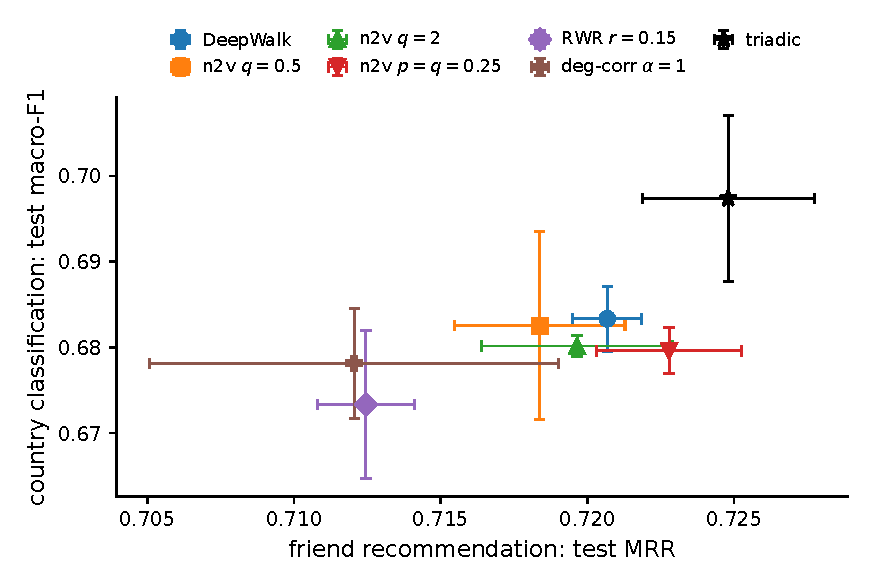
\includegraphics[width=0.78\textwidth]{fig_p1_tradeoff.pdf}
\caption{Each strategy on both tasks at once; error bars are $\pm 1$ sd over the three
seeds.  There is no trade-off frontier --- the triadic walk sits alone in the top-right
corner.}
\label{p1:fig:tradeoff}
\end{figure}

\paragraph{Per-source-degree breakdown.}
Table~\ref{p1:tab:degree} gives \texttt{breakdown\_by\_source\_degree} on the test split for
the baseline and the best strategy; Figure~\ref{p1:fig:degree} adds the worst one.

\begin{table}[H]
\centering\small
\caption{\texttt{breakdown\_by\_source\_degree}, test split, seed $0$, by number of friends
the \emph{source} user has in $G_{\mathrm{train}}$.}
\label{p1:tab:degree}
\begin{tabular}{@{}lccccc@{}}
\toprule
 & & \multicolumn{2}{c}{DeepWalk} & \multicolumn{2}{c}{triadic} \\
\cmidrule(lr){3-4}\cmidrule(lr){5-6}
source degree & $n$ & Hit@1 & MRR & Hit@1 & MRR \\
\midrule
$0$ (cold) & 216 & 0.0833 & 0.2117 & 0.0231 & 0.1756 \\
$1$ & 266 & 0.4511 & 0.5697 & 0.4436 & 0.5676 \\
$2$--$3$ & 469 & 0.5672 & 0.6823 & 0.5586 & 0.6776 \\
$4$--$7$ & 842 & 0.6556 & 0.7656 & 0.6639 & 0.7696 \\
$8$--$15$ & 939 & 0.6784 & 0.7906 & 0.6869 & 0.7947 \\
$\ge 16$ & 1439 & 0.6386 & 0.7677 & 0.6477 & 0.7739 \\
\bottomrule
\end{tabular}
\end{table}

\begin{figure}[H]
\centering
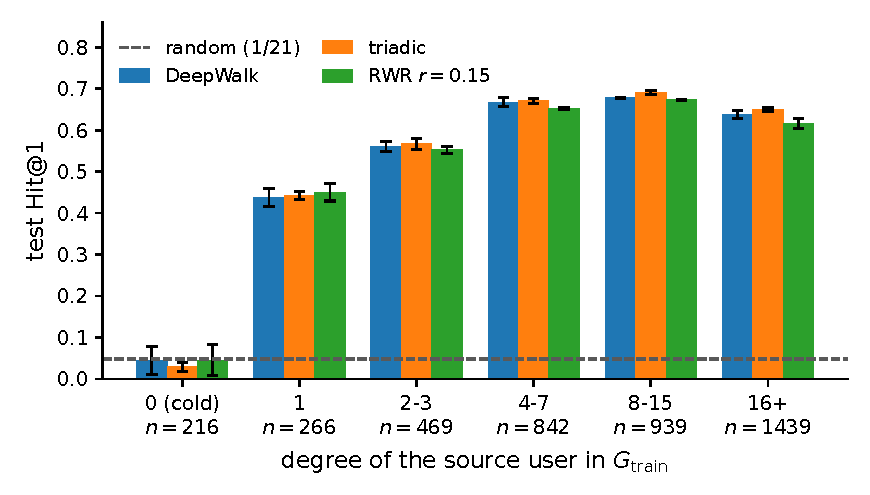
\includegraphics[width=0.82\textwidth]{fig_p1_degree.pdf}
\caption{Test Hit@1 by source degree for the baseline (DeepWalk), the best strategy
(triadic) and the worst (RWR); error bars are $\pm 1$ sd over seeds $\{0,1,2\}$.  The
cold-start bucket sits at chance for every strategy.}
\label{p1:fig:degree}
\end{figure}

\paragraph{Control.}
To check that the evaluation path itself carries no signal, I ran the identical pipeline
on a random Gaussian $Z$: it gives test Hit@1 $0.0671$ and MRR $0.2009$ (chance is
$1/21=0.0476$ and $0.1736$) and country test micro-F1 $0.1340$, far below the
majority-class rate of $0.2062$.  The learned embeddings are therefore genuinely doing
the work.

\subsection{Analysis}
\label{p1:sec:analysis}

\paragraph{The same embedding wins both tasks.}
The triadic walk is best in \emph{every} column of Table~\ref{p1:tab:comparison}, and
Figure~\ref{p1:fig:tradeoff} shows it alone in the top-right corner: there is no
homophily-versus-structural-equivalence trade-off to negotiate on this dataset.  That is
not an accident of the metrics --- both downstream tasks on this graph are homophily
tasks.  Friends of a user are found inside their community, and country is an extremely
assortative label on a social network (people mostly follow people in their own country),
so an embedding that sharpens community boundaries helps the link predictor and the
country classifier for the same reason.  A dataset where node labels were a function of
\emph{role} rather than community (bridges, hubs, peripherals) is where one would expect
the two tasks to pull apart, and where a $q>1$ walk should have paid off.

\paragraph{Which differences are real.}
Most of them are small, so the noise floor matters.  The between-strategy spread is
$4.2\times$ the within-strategy sd for test MRR and $3.9\times$ for test macro-F1 --- real
effects.  But for country \emph{micro}-F1 the spread is only $1.7\times$ the noise
($0.7607$--$0.7661$): \textbf{on micro-F1 the seven strategies are statistically
indistinguishable.}  Anyone reading only the micro-F1 column would conclude that the
sampling strategy does not matter; the macro-F1 column, where the spread is $0.0240$,
shows that it does.  This is exactly the imbalance effect the question points at: the
label distribution runs from $1{,}572$ users in the largest country to $16$ in the
smallest (only $2$ of which land in the $763$-user training split), so micro-F1 is
dominated by a handful of big classes that every embedding already gets right, and only
macro-F1 is sensitive to what happens in the tail.

\paragraph{node2vec buys nothing here.}
All three $(p,q)$ settings sit within noise of plain DeepWalk (test MRR $0.7184$,
$0.7196$, $0.7228$ versus $0.7207$), and the homophily-leaning setting $q{=}0.5$ is if
anything the \emph{worst} of the three.  I read this as a property of the graph rather
than of node2vec: with mean degree $5.1$ and $734$ components, a length-$40$ uniform walk
is already confined to a small neighbourhood, so re-weighting second-order transitions
has little room to change which nodes co-occur.  The second-order machinery costs a
doubling of sampling time and returns nothing measurable.

\paragraph{Why triadic works and the other two ideas do not.}
The triadic rule, $P(x)\propto 1+|N(v)\cap N(x)|$, prefers steps that close a triangle.
It is the only one of my three ideas that adds \emph{new information} --- it looks at the
graph two hops out, whereas uniform, RWR and degree-corrected walks only ever consult the
current node's neighbour list.  That extra information is precisely a community signal,
which is why its largest single gain is country macro-F1 ($0.6974$ vs $0.6833$, $+0.014$,
$2.3$ noise-sds).
\begin{itemize}\itemsep1pt
\item \textbf{RWR was my worst idea} (test MRR $0.7124$, $-0.0083$ against DeepWalk).  The
hypothesis --- that a personalised context sharpens pairwise proximity --- is falsified.
With a fixed length-$40$ budget, teleporting home $15\%$ of the time spends about six
tokens per walk re-emitting \texttt{start} and truncates the walk's effective reach, so
the corpus contains fewer distinct co-occurrences for the same cost.  The breakdown
localises the damage precisely: degree $1$ is the \emph{only} bucket where RWR beats
DeepWalk ($0.4499$ vs $0.4386$ test Hit@1, the largest degree-$1$ gain of any strategy ---
a short leash is exactly right when the source has one friend), and it is worse at every
degree $\ge 2$, by $-0.0218$ in the $\ge 16$ bucket.
\item \textbf{Degree-corrected sampling also failed} (test MRR $0.7121$, $-0.0086$) --- and
failed in an informative way.  The hypothesis was that suppressing hubs would lift the
\emph{low}-degree buckets; the measurement says the opposite happened.  It helped the
high-degree end ($+0.0099$ at $8$--$15$, $+0.0019$ at $\ge 16$) and did its worst damage
at $2$--$3$ ($-0.0199$).  Hubs are not noise to be corrected away: on a social graph a
shared popular contact is real evidence that two users belong together, and re-weighting
by $\deg(x)^{-1}$ discards exactly that evidence --- which hurts most for the sparse users
who had little other evidence to begin with.
\end{itemize}

\paragraph{Cold start is the real bottleneck, and no walk strategy can touch it.}
The single largest effect in this study is not a strategy at all.  Test Hit@1 runs from
$\approx 0.03$ at source degree $0$ to $\approx 0.69$ at degree $8$--$15$ --- a gap of
$0.65$, roughly fifty times the $0.013$ that separates the best strategy from the worst.
The $666$ isolated users have no incident edge in $G_{\mathrm{train}}$, so
\texttt{sample\_walks} correctly returns \texttt{[]} for them and their embedding row is
zero \emph{by construction}.  The $216$ test queries with such a source are therefore
being scored from destination-side features alone, and the numbers confirm it exactly:
the cold bucket's seed-averaged Hit@1/MRR ($0.0447/0.1887$ for DeepWalk) match the
random-$Z$ control ($0.0671/0.2009$) and chance ($0.0476/0.1736$) rather than any learned
result.  Across all $21$ runs that bucket wanders between $0.0139$ and $0.1065$ with no
strategy stable across its own three seeds --- DeepWalk alone scores $0.0833$, $0.0231$,
$0.0278$ --- so it is pure tie-breaking noise on $216$ queries.  Reading the cold-start
column as evidence about a sampling strategy would be a mistake.  Fixing it
requires information from outside the observed social graph --- structural or profile
features, or the user--artist edges used in Task 4 --- not a better walk.

\paragraph{The non-monotone top bucket.}
Hit@1 peaks at degree $8$--$15$ and falls back for $\ge 16$ (seed-averaged
$0.6904 \to 0.6502$ for triadic).  More friends means more embedding evidence but also a
harder ranking problem: a high-degree user is plausibly connected to many of the $20$
sampled negatives, so the single held-out positive is genuinely harder to place first.
MRR falls much less than Hit@1 ($0.7959\to0.7744$), consistent with the positive still
being ranked near the top rather than lost.  These two top buckets are also where triadic
beats DeepWalk by the widest margin ($+0.0121$ and $+0.0125$ Hit@1, against $+0.0038$ at
degree $1$), which fits the same story: for a hub user, knowing \emph{which} community a
candidate belongs to is what separates the true friend from a plausible negative.

\paragraph{Practical conclusion.}
If I had to ship one embedding for both products, it would be the triadic walk: it is the
best on both tasks, it is first-order (so it is as cheap to sample as DeepWalk once the
edge weights are precomputed, $1.9$\,s versus $0.7$\,s for the whole corpus, against
$1.3$\,s for node2vec), and it needs no $(p,q)$ tuning.  But the honest headline is that
on this graph the choice of random-walk strategy moves test MRR by about $1.3$ points at
most, while the degree of the query user moves it by $65$; effort is better spent on the
cold-start population than on the sampler.
